\subsubsection{评价结果}

根据上述指标计算各十年区间相对于前一区间的气温增幅，结果如图~\ref{fig:q1a-annual-increase} 所示。可以发现，不同时期的气温增幅存在差异，既有升温区间，也有降温区间，而近年来整体表现为升温。

其中，2013---2022年的平均气温较2003---2012年上升约 $0.25\,{}^\circ\mathrm{C}$，是所划分区间中的最高增幅。这说明最近十年的平均气温上升幅度超过了此前各分组区间，支持近期全球增暖更加明显的判断。

\begin{figure}[htbp]
    \centering
    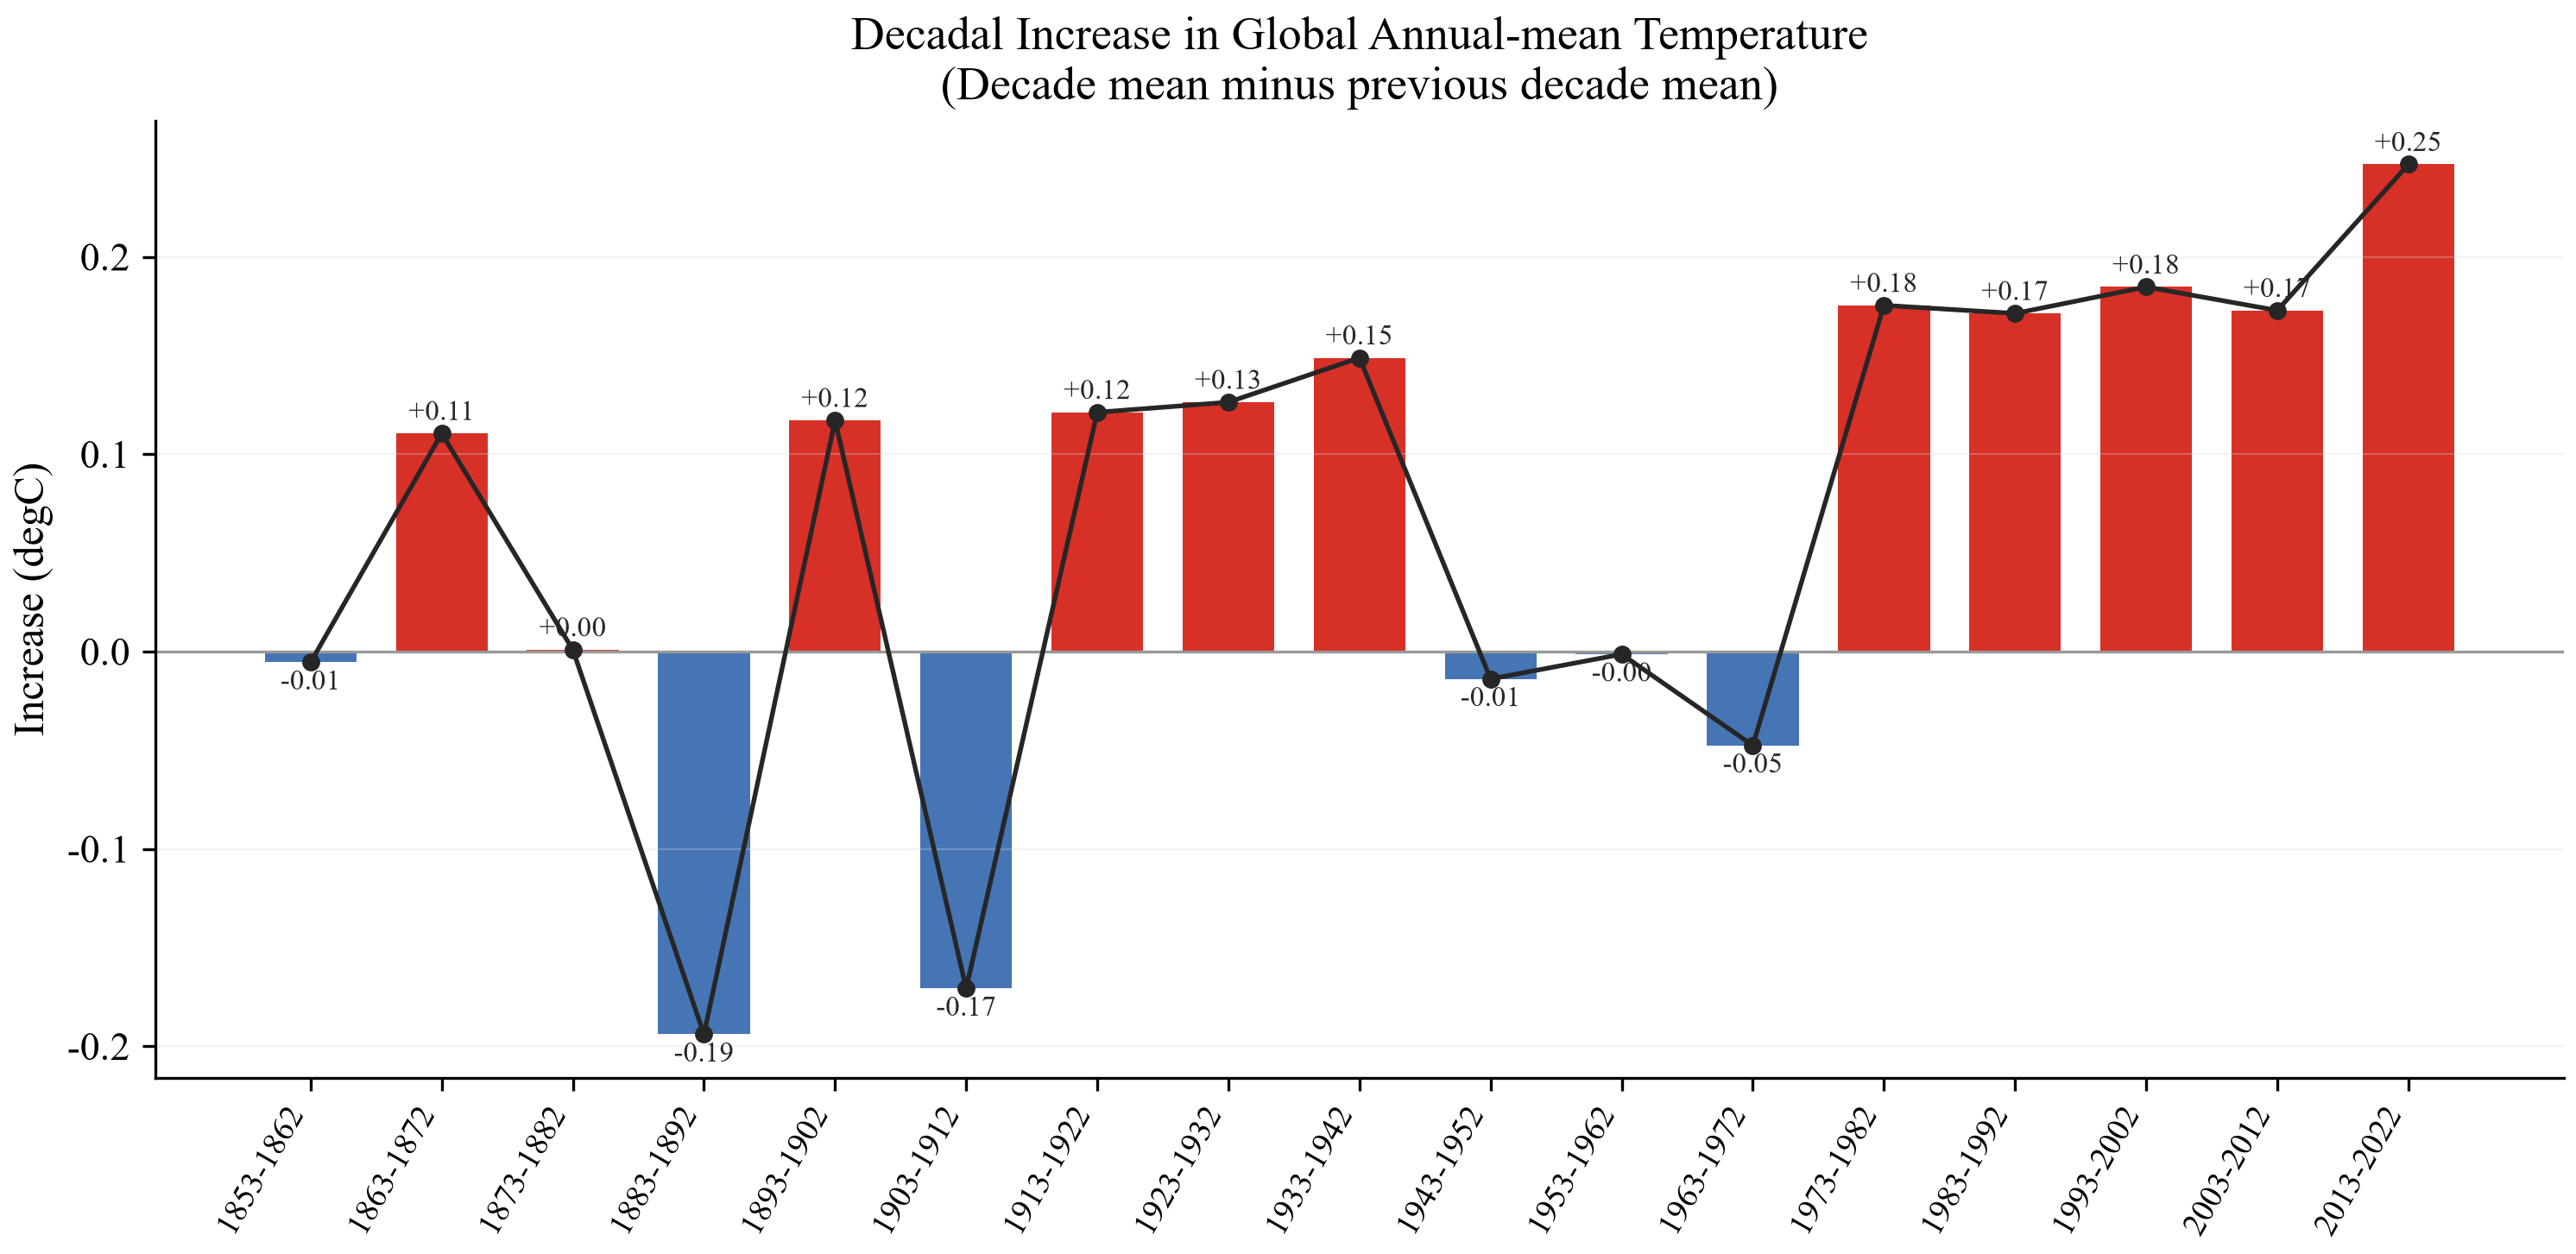
\includegraphics[width=0.85\textwidth]{../image/Q1/annual_temperature_increase.png}
    \caption{全球年均气温的十年增幅}
    \label{fig:q1a-annual-increase}
\end{figure}
